\section{Angular Kinematics}

In this lab you will explore the relationships between mass distributions, torques, angular momentum, and angular kinematics.
\hfill \break

Open Interactive Physics, turn gravity off, and create a T-shaped rotational object as shown.
Keep the thickness reasonably small.
You will have to attach the object to an anchor using a ``pin joint'' and attach the two parts of the T together with ``rigid joints.''
%
\begin{figure}[H]
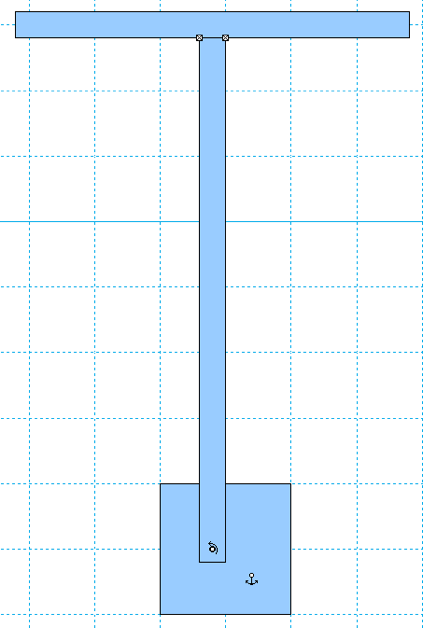
\includegraphics[scale=0.70]{figures/angularKinematics/figure1.png}
\end{figure}
%

\underline{\textbf{Part 1}} \par
Calculate the moment of inertia of the object about the base of the T.
Use the torque tool to apply a torque to the base of the T.
Measure the angular acceleration of the object for at least 4 values of torque.
Create a plot of $\alpha$ vs $\uptau$ and use this data to extract the object's moment of inertia.
Compare the result to your calculation.
\hfill \break

\underline{\textbf{Part 2}} \par
For a fixed value of torque, measure $\omega_i$ and $\omega_f$ over some time interval $\Delta t$.
Use this data to show that $\uptau = \Delta L / \Delta t$.
Repeat for a different value of torque.

\pagebreak \clearpage
